\documentclass[12pt]{article}
\usepackage{amsmath, amssymb, amsthm, enumerate, graphicx}
\usepackage[usenames,dvipsnames]{color}
\usepackage{bm}
\usepackage[colorlinks=true,urlcolor=blue]{hyperref}
\usepackage{geometry}
\geometry{margin=1in}
\usepackage{float}
\usepackage{graphics}
\setlength{\marginparwidth}{2.15cm}
\usepackage{booktabs}
\usepackage{enumitem}
\usepackage{epsfig}
\usepackage{setspace}
\usepackage{parskip}
\usepackage[normalem]{ulem}
\usepackage{tikz}
\usetikzlibrary{positioning, arrows, automata}
\usepackage{pgfplots}
\usepackage[font=scriptsize]{subcaption}
\usepackage{float}
\usepackage[]{algorithm2e}
\usepackage{environ}
\usepackage{bbm}
\usepackage{graphicx}
\usepackage{titling}
\usepackage{url}
\usepackage{xcolor}
\usepackage{lipsum}
\usepackage{lastpage}
\usepackage[colorlinks=true,urlcolor=blue]{hyperref}
\usepackage{multicol}
\usepackage{tabularx}
\usepackage{comment}
\usepackage[utf8]{inputenc}
\usepackage{amssymb}
\usepackage{setspace}
\usepackage{marvosym}
\usepackage{wrapfig}
\usepackage{datetime}
\usepackage[many]{tcolorbox}
\usepackage{array}
\usepackage{multirow}
\usepackage{wasysym}
\usepackage{cancel}

\usepackage{listings}
\usepackage{color}


\newcommand{\R}{\mathbb{R}}
\newcommand{\blackcircle}{\tikz\draw[black,fill=black] (0,0) circle (1ex);}
\renewcommand{\circle}{\tikz\draw[black] (0,0) circle (1ex);}


% SOLUTION environment
\NewEnviron{soln}{
\leavevmode\color{red}\ignorespaces \textbf{Solution} \BODY }{}

% QUESTION AUTHORS environment
\NewEnviron{qauthor}{
\leavevmode\color{blue}\ignorespaces \textbf{Author} \BODY}{}

% TO ONLY SHOW HOMEWORK QUESTIONS, include following (else comment out):
\RenewEnviron{soln}{}
%\RenewEnviron{qauthor}{}


%\newcommand{\norm}[1]{\lVert #1 \rVert}
%\newcommand{\st}{\mathrm{s.t.}}

\makeatletter
\newcommand{\removelatexerror}{\let\@latex@error\@gobble}
\makeatother

\newcommand{\argmax}{\mathop{\mathrm{argmax}}}
\newcommand{\argmin}{\mathop{\mathrm{argmin}}}


%%%%%%%%%%%%%%%%%%%%%%%%%%%%%%%%%%%%%%%%%%%
% Custom box for highlights               %
%%%%%%%%%%%%%%%%%%%%%%%%%%%%%%%%%%%%%%%%%%%

% Define box and box title style
\tikzstyle{mybox} = [fill=blue!10, very thick,
    rectangle, rounded corners, inner sep=1em, inner ysep=1em]

% \newcommand{\notebox}[1]{
% \begin{tikzpicture}
% \node [mybox] (box){%
%     \begin{minipage}{\textwidth}
%     #1
%     \end{minipage}
% };
% \end{tikzpicture}%
% }

\NewEnviron{notebox}{

\begin{tikzpicture}
\node [mybox] (box){
    \begin{minipage}{\textwidth}
        \BODY
    \end{minipage}
};
\end{tikzpicture}
}


\begin{document}

\section*{}
\begin{center}
  \centerline{\textsc{\LARGE  Homework 1}}
  \vspace{0.5em}
  \centerline{\textsc{\LARGE Background}\footnote{Compiled on \today{} at \currenttime{}}}
  \vspace{1em}
  \textsc{\large CMU 10-601: Machine Learning (Fall 2018)} \\
  \vspace{0.5em}
  \url{piazza.com/cmu/fall2018/10601bd} \\
  \vspace{0.5em}
  \centerline{OUT: Wednesday, Aug 29th, 2018}
  %\today{} at \currenttime{}}}
  \vspace{0.5em}
  \centerline{DUE: Wednesday, Sept 5th, 2018, 11:59pm}
    \centerline{TAs: Rongye Shi, Sida Gao, Rawal Khirodkar, George Xu}
\end{center}


\section*{START HERE: Instructions}
\begin{itemize}
\item \textbf{Collaboration policy:} Collaboration on solving the homework is allowed, after you have thought about the problems on your own. It is also OK to get clarification (but not solutions) from books or online resources, again after you have thought about the problems on your own. There are two requirements: first, cite your collaborators fully and completely (e.g., ``Jane explained to me what is asked in Question 2.1''). Second, write your solution {\em independently}: close the book and all of your notes, and send collaborators out of the room, so that the solution comes from you only.  See the Academic Integrity Section on the course site for more information: \url{http://www.cs.cmu.edu/~mgormley/courses/10601bd-f18/about.html#7-academic-integrity-policies}

\item\textbf{Late Submission Policy:} See the late submission policy here: \url{http://www.cs.cmu.edu/~mgormley/courses/10601bd-f18/about.html#6-general-policies}

\item\textbf{Submitting your work:} 

\begin{itemize}

% Since we are not using Canvas this semester.
% \item \textbf{Canvas:} We will use an online system called Canvas for short answer and multiple choice questions. You can log in with your Andrew ID and password. (As a reminder, never enter your Andrew password into any website unless you have first checked that the URL starts with "https://" and the domain name ends in ".cmu.edu" -- but in this case it's OK since both conditions are met).  You may only \textbf{submit once} on canvas, so be sure of your answers before you submit.  However, canvas allows you to work on your answers and then close out of the page and it will save your progress.  You will not be granted additional submissions, so please be confident of your solutions when you are submitting your assignment.

\item \textbf{Autolab:} You will submit your code for programming questions on the homework to Autolab (\url{https://autolab.andrew.cmu.edu/}). After uploading your code, our grading scripts will autograde your assignment by running your program on a virtual machine (VM). The software installed on the VM is identical to that on \texttt{linux.andrew.cmu.edu}, so you should check that your code runs correctly there. If developing locally, check that the version number of the programming language environment and versions of permitted libraries match those on linux.andrew.cmu.edu. (Octave users: Please make sure you do not use any Matlab-specific libraries in your code that might make it fail against our tests.) You have a \textbf{total of 10 Autolab submissions.} Use them wisely. In order to not waste Autolab submissions, we recommend debugging your implementation on your local machine (or the linux servers) and making sure your code is running correctly first before any Autolab submission. {\color{red} The above is true for future assignments, but this one allows \textbf{unlimited submissions.}}

\item \textbf{Gradescope:} For written problems such as short answer, multiple choice, derivations, proofs, or plots, we will be using Gradescope (\url{https://gradescope.com/}). Please use the provided template. Submissions can be handwritten onto the template, but should be labeled and clearly legible. If your writing is not legible, you will not be awarded marks. Alternatively, submissions can be written in LaTeX. Regrade requests can be made, however this gives the TA the opportunity to regrade your entire paper, meaning if additional mistakes are found then points will be deducted.
Each derivation/proof should be  completed on a separate page. {\color{red} For this assignment only, if you answer at least 90\% of the written questions correctly, you get full marks on the Gradescope portion of this assignment. For this assignment only, \textbf{we will offer two rounds of grading}. The first round of grading will happen immediately following the due date specified above. We will then release your grades to you and if you got less than 90\% on the written questions, you will be allowed to submit once again by a second due date. The exact due date for the second round will be announced after we release the first round grades. }

\end{itemize}

\item \textbf{Materials:} Download from autolab the tar file (``Download handout"). The tar file will contain all the data that you will need in order to complete this assignment.

\end{itemize}

%Homework 9 will be on Gradescope, but will be "Canvas-style"- all problems will be multiple choice, select all that apply, or numerical answer. 

For multiple choice or select all that apply questions, shade in the box or circle in the template document corresponding to the correct answer(s) for each of the questions. For \LaTeX users, use $\blacksquare$ and \blackcircle  for shaded boxes and circles, and don't change anything else.



\clearpage

%\clearpage
\section{Hello, Autolab! [38 Points]} 

\subsection{Introduction}

This homework is neither representative the standard difficulty of programming assignments for this course nor is it designed to test your ability to program. \textbf{In this homework you have to choose Python, Octave, Java, or C++ as your programming language. Submitting code for more than one language may result in undefined behavior..}

The goal of this assignement is to ensure that you:
\begin{enumerate}
    \item Have a way to edit and test your code (i.e. a text editor and compiler/interpreter)
    \item Are familiar with submitting to Autolab
    \item Are familiar with file I/O and standard output in the language of your choice
\end{enumerate}

\textbf{Warning:} This handout assumes that you are using a unix command prompt (with \texttt{zsh, bash, csh} or similar). All of the command prompts lines listed in this handout will work on the linux.andrew.cmu.edu machines. You may need to use other commands or methods if you are working locally - especially if you are using Windows.

\subsection{Reading from a file [30pts]}

In \texttt{reverse.\{py|m|java|cpp\}}, implement a program that reads in the lines of a file, then writes them in reverse order to an output file. Specifically, your program should take two command line arguments: the name of the input file and the name of the output file. It should read the lines of the input file and write them to the output file from last to first, separated by ``\textbackslash n". You should assume that the input file has unix-style line breaks. (Windows uses ``\textbackslash r\textbackslash n" to indicate a new line. Unix uses only ``\textbackslash n".)

For example, if the file \texttt{input.txt} contained the stream

\begin{verbatim}
    #pineapples\n#pinstripes\n#pinwheelofdoom\n#pinsir\n
\end{verbatim}

which is commonly displayed as
\begin{verbatim}
    #pineapples
    #pinstripes
    #pinwheelofdoom
    #pinsir
\end{verbatim}

depending on your language of choice, one of the following:

\begin{itemize}
    \item \texttt{python reverse.py input.txt output.txt}
    \item \texttt{octave -qH reverse.m input.txt output.txt}
    \item \texttt{javac reverse.java; java reverse input.txt output.txt}
    \item \texttt{g++ reverse.cpp; ./a.out input.txt output.txt}
\end{itemize}

should write the following to output.txt

\begin{verbatim}
    #pinsir\n#pinwheelofdoom\n#pinstripes\n#pineapples\n
\end{verbatim}

which is displayed as

\begin{verbatim}
    #pinsir
    #pinwheelofdoom
    #pinstripes
    #pineapples
\end{verbatim}

You may assume that the contentes of the input file will fit in memory for any reasonable machine and the contents of the file will be ASCII-encoded. You will be provided with two example files \texttt{example.txt} and \texttt{sentences.txt} with which you can test your code. However, do not assume that if your code works on just those files than it will receive full points. We will grade your code on different, hidden test cases. Attempts to directly determine the specific contents of these tests constitute violation of the course policy.

{\color{red} 
Note to Octave users: Please be sure that \texttt{reverse.m} is a \textit{script} that gets its arguments from the command line rather than a \textit{function}.}

\subsection{Test Code on \texttt{linux.andrew.cmu.edu} Machines}

Before submitting to Autolab on this and \textbf{every future assignment}, you should check that it behaves correctly when run on the \texttt{linux.andrew.cmu.edu} machines, since they mirror the software installed on the Autolab virtual machines (VMs). These instructions assume you are working on a unix based operating system (e.g. Linux, Mac OS) - if you are using Windows you can install cygwin (\url{https://www.cygwin.com/}) which provides a unix-like environment. (Of course, you are also welcome to develop your code directly on these same servers.)

Follow the three stpes below. Here we assume your code and the \texttt{example.txt} file are located in a subdirectory \texttt{./reverse/}.

\begin{enumerate}
    \item Copy your code to the linux server:
    \begin{verbatim}
    rsync -a ./reverse/ <Your Andrew ID>@linux.andrew.cmu.edu:~/reverse/\end{verbatim}
    
    \item Log into the linux server:
    \begin{verbatim}
    ssh <Your Andrew ID>@linux.andrew.cmu.edu\end{verbatim}
    
    \item Change directories to where you just copied the code:
    \begin{verbatim}
    cd  ~/reverse/\end{verbatim}
    
    \item Run the code with one of the below:
    \begin{itemize}
        \item \texttt{python reverse.py example.txt output.txt}
        \item \texttt{octave -qH reverse.m example.txt output.txt}
        \item \texttt{javac reverse.java; java reverse example.txt output.txt}
        \item \texttt{g++ -g -std=c++11 reverse.cpp; ./a.out example.txt output.txt}
    \end{itemize}
    
    \item Check that it was properly reversed:
    \begin{verbatim}
    cat output.txt\end{verbatim}
\end{enumerate}

\subsection{Autolab Submission [8pts]}

You must submit a .tar file named \texttt{reverse.tar} containing \texttt{reverse.\{py|m|java|cpp\}}. You can create that file by running:
\begin{verbatim}    tar -cvf reverse.tar reverse.{py|m|java|cpp}\end{verbatim}

from the directory containing your code.

Some additional tips: \textbf{DO NOT} compress your files; you are just creating a tarball. Do not use tar \texttt{-czvf}. \textbf{DO NOT} put the above files in a folder and then tar the folder. Autolab is case sensitive, so observe that all your files should be named in \textbf{lowercase}. You must submit this file to the corresponding homework link on Autolab.

Note: For this assignment, you may make arbitrarily many submissions to Autolab before the deadline, but only your last submission will be graded.


 \begin{notebox}
  {\bf Python3 Users:} Please include a blank file called python3.txt (case-sensitive) in your tar submission and we will execute your submitted program using Python 3 instead of Python 2.7. If the file is not present, we will default to running your code with Python 2.7.
 \end{notebox}


\clearpage

\section*{Instructions for Specific Problem Types}

For ``Select One" questions, please fill in the appropriate bubble completely:

\begin{quote}
\textbf{Select One:} Who taught this course?
\begin{list}{}
     \item\CIRCLE{} Matt Gormley
     \item\Circle{} Marie Curie
     \item\Circle{} Noam Chomsky
\end{list}
\end{quote}

If you need to change your answer, you may cross out the previous answer and bubble in the new answer:

\begin{quote}
\textbf{Select One:} Who taught this course?
\begin{list}{}
     \item\CIRCLE{} Matt Gormley
     \item\Circle{} Marie Curie\\
     \xcancel{\CIRCLE}{} Noam Chomsky
\end{list}
\end{quote}


For ``Select all that apply" questions, please fill in all appropriate squares completely:

\begin{quote}
\textbf{Select all that apply:} Which are scientists?
    \begin{list}{}
    \item $\blacksquare$ Stephen Hawking 
    \item $\blacksquare$ Albert Einstein
    \item $\blacksquare$ Isaac Newton
    \item $\square$ I don't know
\end{list}
\end{quote}

Again, if you need to change your answer, you may cross out the previous answer(s) and bubble in the new answer(s):

\begin{quote}
\textbf{Select all that apply:} Which are scientists?
    \begin{list}{}
    \item $\blacksquare$ Stephen Hawking 
    \item $\blacksquare$ Albert Einstein
    \item $\blacksquare$ Isaac Newton\\
    \xcancel{$\blacksquare$} I don't know
\end{list}
\end{quote}

For questions where you must fill in a blank, please make sure your final answer is fully included in the given space. You may cross out answers or parts of answers, but the final answer must still be within the given space.

\begin{quote}
\textbf{Fill in the blank:} What is the course number?

\begin{tcolorbox}[fit,height=1cm, width=4cm, blank, borderline={1pt}{-2pt},nobeforeafter]
    \begin{center}\huge10-601\end{center}
    \end{tcolorbox}\hspace{2cm}
    \begin{tcolorbox}[fit,height=1cm, width=4cm, blank, borderline={1pt}{-2pt},nobeforeafter]
    \begin{center}\huge10-\xcancel{7}601\end{center}
    \end{tcolorbox}
\end{quote}



\section{Prerequisite Practice[62 Points]}

In this section, you will work through a number of problems covering probability, statistics, calculus, linear algebra, geometry, and computer science. 

\subsection{Probability and Statistics [30pts]}

\textbf{\underline{Use the following data to answer questions 1-4}}. Consider data created by flipping a coin five times $S $ = [1, 1, 0, 1, 1] , where 1 denotes that the coin turned up heads and 0 denotes that it turned up tails. \bigskip

\begin{enumerate}
    \item \textbf{[2pt]} The sample mean for this data is:
    
    \textbf{Select one:}
    \begin{list}{}
        \item $\circle$ 1
        \item $\circle$ $\frac{3}{5}$
        \item $\circle$ $\frac{1}{5}$
        \item $\circle$ $\frac{4}{5}$
    \end{list}


    \item \textbf{[2pt]} The (uncorrected) sample variance for this data is:

    \textbf{Select one:}
    \begin{list}{}
        \item $\circle$ $\frac{1}{25}$
        \item $\circle$ $\frac{2}{25}$
        \item $\circle$ $\frac{4}{25}$
        \item $\circle$ $\frac{8}{25}$
    \end{list}


    \item \textbf{[2pt]} With reference to the previous question, what is the probability of observing this data, assuming it was generated by flipping a coin X with an unequal probability of heads (1) and tails (0), where now the distribution is $P(X = 1) = 0.75$, $P(X = 0) = 0.25$?

    \textbf{Select one:}
    \begin{list}{}
        \item $\circle$ $\frac{1}{1024}$
        \item $\circle$ $\frac{1}{32}$
        \item $\circle$ $\frac{9}{1024}$
        \item $\circle$ $\frac{81}{1024}$
    \end{list}


    \item \textbf{[2pt]} Note that the probability of this data sample would be greater if the value of P(X = 1) was not 0.5, but instead some other value. What is the value that maximizes the probability of the sample S?

    \textbf{Select one:}
    \begin{list}{}
        \item $\circle$ $\frac{4}{5}$
        \item $\circle$ $\frac{1}{5}$
        \item $\circle$ 1
        \item $\circle$ $\frac{3}{5}$
    \end{list}


    \item \textbf{[2pt]} State true or false.  For events A and B, $$ P(A \cap B) = P(A) + P(B) - P(A \cup B)$$

    \textbf{Select one:}
    \begin{list}{}
        \item $\circle$ True
        \item $\circle$ False
    \end{list}


    \item \textbf{[2pt]} State true or false. For events A and B, $$P(A_1\cap A_2 \cap A_3) = P(A_3|A_2\cap A_1)P(A_2|A_1)P(A_1)$$

    \textbf{Select one:}
    \begin{list}{}
        \item $\circle$ True
        \item $\circle$ False
    \end{list}

    
    
    \bigskip\bigskip\bigskip
    \textbf{\underline{Use the following information to answer questions 7-8}}. Whether your car is wet in the morning (W) is dependent on whether it rained last night (R) or not, however other factors may have lead to your car being wet. The following are probabilities of such events:
    \begin{eqnarray*}
        & P(R) = 0.4\\
        & P(W | R) = 0.8\\
        & P(W | \neg R ) = 0.2
    \end{eqnarray*}
    

    \item \textbf{[2pt]} What is the probability of $P(\neg R)$?
(Here $ \neg R$ reads: no rain last night)

    \textbf{Select one:}
    \begin{list}{}
        \item $\circle$ 0.1
        \item $\circle$ 0.4
        \item $\circle$ 0.9
        \item $\circle$ 0.6
    \end{list}


    \item \textbf{[2pt]} Using the same probabilities as the previous question, what is the probability that your car is wet in the morning?

    \textbf{Select one:}
    \begin{list}{}
        \item $\circle$ 0.64
        \item $\circle$ 0.56
        \item $\circle$ 0.44
        \item $\circle$ 0.4
    \end{list}

    
    \bigskip\bigskip\bigskip
    \textbf{\underline{Use the following information to answer questions 9-10}}. Consider the following joint probability table where both X and Y are binary variables:\\[12pt] 
    \begin{tabular}{ccc}
    X & Y & Probability \\
    0 & 0 & 0.1\\
    0 & 1 & 0.2\\
    1 & 0 & 0.4\\
    1 & 1 & 0.3
    \end{tabular}


    \item \textbf{[2pt]} Using the same table, what is $P(X = 1 | Y=1)$?

    \textbf{Select one:}
    \begin{list}{}
        \item $\circle$ $\frac{2}{3}$
        \item $\circle$ $\frac{3}{7}$
        \item $\circle$ $\frac{4}{5}$
        \item $\circle$ $\frac{3}{5}$
    \end{list}


    \item \textbf{[2pt]} What is $P(Y=0)$?

    \textbf{Select one:}
    \begin{list}{}
        \item $\circle$ 0.2
        \item $\circle$ 0.6
        \item $\circle$ 0.5
        \item $\circle$ 0.3
    \end{list}

    
    
    \bigskip\bigskip\bigskip
    \textbf{\underline{Use the following information to answer questions 11-13}}. Let X be a random variable and the expected value of X is $E[X] = 1$ and the variance of X is $Var[X] = 1$. 

    \item \textbf{[2pt]} What is $E[6X]$?

    \textbf{Select one:}
    \begin{list}{}
        \item $\circle$ 1
        \item $\circle$ 3
        \item $\circle$ 6
        \item $\circle$ 36
    \end{list}


    \item \textbf{[2pt]} What is $Var[3X]$?

    \textbf{Select one:}
    \begin{list}{}
        \item $\circle$ 1
        \item $\circle$ 3
        \item $\circle$ 6
        \item $\circle$ 9
    \end{list}


    \item \textbf{[2pt]} What is $Var[2X + 3]$?

    \textbf{Select one:}
    \begin{list}{}
        \item $\circle$ 3
        \item $\circle$ 4
        \item $\circle$ 5
        \item $\circle$ 7
    \end{list}


    \item \textbf{[2pt]} What is the mean, variance and entropy of a Bernoulli (p) random variable?
    
    \textbf{Select one:}
    \begin{list}{}
        \item $\circle$ $p, p(1-p), -(1-p)\log(1-p)-p \log(p)$
        \item $\circle$ $p(1-p), p, -(1-p)\log(1-p)-p\log(p)$
        \item $\circle$ $p, -(1-p)\log(1-p)-p\log(p), p(1-p)$
        \item $\circle$ The entropy of a Bernoulli variable is not defined.
    \end{list}
    

    \item \textbf{[2pt]} Please match the probability density function of the random variable X to its corresponding distribution name.
    
    \begin{enumerate}
        \item  prob(X=x) = $\frac{1}{\sqrt{(2\pi)^d |\sum|}}\exp(-\frac{1}{2}(x - \mu)^T\sum^{-1}(x-\mu))$
        \item  prob(X=x) = $\lambda e^{-\lambda x}$ when $x \geq 0$; 0 otherwise
        \item  prob(X=x) = $\binom{n}{x} p^x (1-p)^{n-x}$
        \item  prob(X=x) = $\frac{1}{b-a}$ when $a \leq x \leq b$; 0 otherwise
        \item  prob(X=x) = $p^x(1-p)^{1-x}$
    \end{enumerate}
    
    \begin{list}{}
        \item Multivariate Gaussian:  \qquad
            \begin{tcolorbox}[fit,height=1cm, width=2cm, blank, borderline={1pt}{-2pt},nobeforeafter]
            %solution
            \end{tcolorbox}
        \item Exponential:  \qquad
            \begin{tcolorbox}[fit,height=1cm, width=2cm, blank, borderline={1pt}{-2pt},nobeforeafter]
            %solution
            \end{tcolorbox}
        \item Uniform:  \qquad         
            \begin{tcolorbox}[fit,height=1cm, width=2cm, blank, borderline={1pt}{-2pt},nobeforeafter]
            %solution
            \end{tcolorbox}
        \item Bernoulli:  \qquad             
            \begin{tcolorbox}[fit,height=1cm, width=2cm, blank, borderline={1pt}{-2pt},nobeforeafter]
            %solution
            \end{tcolorbox}
        \item Binomial:  \qquad             
            \begin{tcolorbox}[fit,height=1cm, width=2cm, blank, borderline={1pt}{-2pt},nobeforeafter]
            %solution
            \end{tcolorbox}
    \end{list}

    
    
    
    

    \clearpage
\end{enumerate}

\subsection{CS Foundations [10pts]}
\begin{enumerate}
    \item \textbf{[2pt]} If $f(n)=\ln(n)$ and $g(n)=\log_3(n)$ which of the following are true?

    \textbf{Select one:}
    \begin{list}{}
        \item $\circle$ $f(n)=O(g(n))$
        \item $\circle$ $g(n)=O(f(n))$
        \item $\circle$ Both 
        \item $\circle$ Neither
    \end{list}


    \item \textbf{[2pt]} If $f(n)=n^{10}$ and $g(n)=10^n$ which of the following are true?

    \textbf{Select one:}
    \begin{list}{}
        \item $\circle$ $f(n)=O(g(n))$
        \item $\circle$ $g(n)=O(f(n))$
        \item $\circle$ Both
        \item $\circle$ Neither
    \end{list}


    %\clearpage
    \begin{figure}[H]
        \centering
        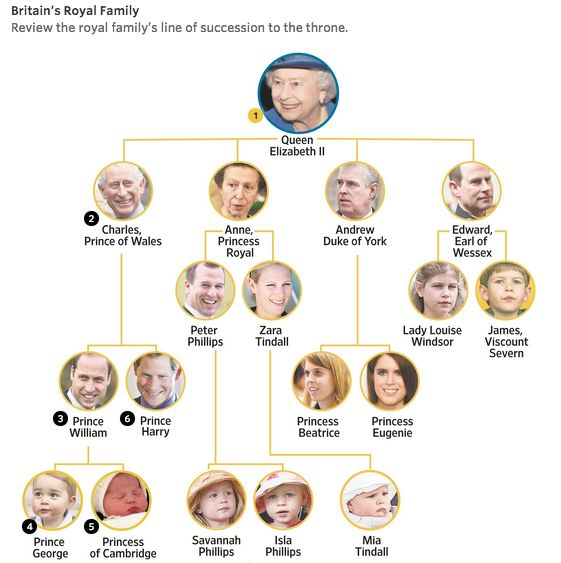
\includegraphics[width=0.6\textwidth]{BritiansRoyalFamily.jpg}
        \caption{Britian's Royal Family}
        \label{Britian's Royal Family}
    \end{figure}
    
    \item \textbf{[2pt]} Using the tree shown above, how many nodes would depth-first-search visit in finding Mia Tindall (including her node)? Assuming we search left-to-right and top-down.

    \textbf{Select one:}
    \begin{list}{}
        \item $\circle$ 3
        \item $\circle$ 12
        \item $\circle$ 15
        \item $\circle$ 18
    \end{list}

    
    %\clearpage
    \begin{figure}[H]
        \centering
        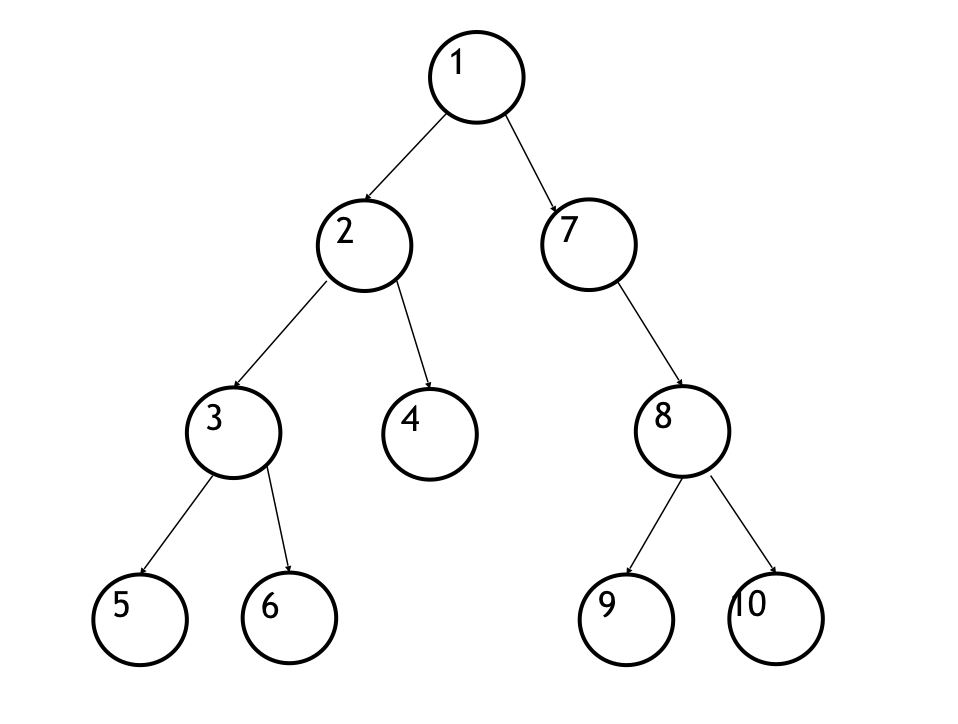
\includegraphics[width = 0.4\textwidth]{TreePlot.png}
        \caption{A Binary Tree with indexed nodes}
        \label{tree}
    \end{figure}
    \item \textbf{[2pt]} Shown above is a Binary Tree with indexed nodes. Assume root node is node 1. What is the node-visit order of \textbf{DFS} and \textbf{BFS} of the above Binary Tree? 
    
    A depth-first search (DFS) traversal of a binary tree starts with visiting the root node, and recursively searches down the left subtree (i.e., the tree rooted at the left node) before going to search the right subtree (i.e., the tree rooted at the right node) until the traversal is done.\\
    Note: Alternatively, we can also look right subtree before left subtree too, for the question please consider left to right order!
    
    A breath-first search (BFS) traversal of a binary tree visits every node (assuming a left-to-right order) on a level (with the same distance to the root) before going to a lower level until the traversal is done.
    
    The node-visit order of DFS is:
    
    \begin{tcolorbox}[fit,height=1cm, width=\textwidth, blank, borderline={1pt}{-2pt},nobeforeafter]
    %solution
    \end{tcolorbox}
    
    The node-visit order of BFS is:
    
    \begin{tcolorbox}[fit,height=1cm, width=\textwidth, blank, borderline={1pt}{-2pt},nobeforeafter]
    %solution
    \end{tcolorbox}
    
    
    \clearpage

    \item \textbf{[2pt]} Fill in the blanks in the pseudo code for key search using recursive depth-first search (DFS) traversal.
    
    \begin{verbatim}
    class TreeNode:
        def __init__(self, val):
            self.val = val
            self.leftNode = None
            self.rightNode = None
        
    # the left/right node is denoted as node.leftNode/node.rightNode
    # left/right node are of type TreeNode
    # the value of the node is denoted as node.val
    # recursive DFS to search for the node with value key in a binary tree
    # the left node is assumed to be searched before the right node
        
    def find_val(node, key):
        if node is None:
            return None
            
        if (1)____________________________:
            return node
            
        else:
            result = (2)___________________________
            
            if result is None:
                result = (3)___________________________
                
            return (4)___________________________
                
    \end{verbatim}
    
    
    

    \clearpage
\end{enumerate}

\subsection{Calculus [8pts]}
\begin{enumerate}
    \item \textbf{[2pt]} Find the derivative of y with respect to x, where $y=2x^3+x-5$

    \textbf{Select one:}
    \begin{list}{}
        \item $\circle$ $6x^2$
        \item $\circle$ $6x^2-5$
        \item $\circle$ $6x^2+1$
        \item $\circle$ $6x^2+x-5$
    \end{list}


    \item \textbf{[2pt]} Evaluate the derivative of y with respect to x, where $y = x^2 + \frac{4}{x^3}$ at x = 1.

    \begin{tcolorbox}[fit,height=1cm, width=2cm, blank, borderline={1pt}{-2pt},nobeforeafter]
    %solution
    \end{tcolorbox}


    \item \textbf{[2pt]} Find the partial derivative of $y$ with respect to $x$, where $y= 3x \cos(z) e^{-x}$

    \textbf{Select one:}
    \begin{list}{}
        \item $\circle$ $3\cos(z) e^{-x}(1-x)$
        \item $\circle$ $3\cos(z) e^{-x}$
        \item $\circle$ $3\cos(z) e^{-x}(1+x)$
        \item $\circle$ $-3\sin(z)e^{-x}$
    \end{list}


    \item \textbf{[2pt]} If you take the derivative of $-x^2 - 4x - 3$ set the derivative to 0 and solve for x you will find:

    \textbf{Select one:}
    \begin{list}{}
        \item $\circle$ a minimum
        \item $\circle$ a maximum
        \item $\circle$ a minimum or a maximum
        \item $\circle$ None of the above
    \end{list}


    \clearpage
\end{enumerate}


\subsection{Vectors and Matrices [8pts]}
\begin{enumerate}
    \item \textbf{[2pt]} Consider the matrix X and the vectors y and z below: X=$\begin{bmatrix} 1 & 4 \\ 2 & 6 \end{bmatrix}$ y=$\begin{bmatrix} 2 \\ 1 \end{bmatrix}$ z=$\begin{bmatrix} 2 \\ 3 \end{bmatrix}$ What is the inner product of the vectors y and z? (this is also sometimes called the dot product)

    \textbf{Select one:}
    \begin{list}{}
        \item $\circle$ $\begin{bmatrix} 14 \\ 22 \end{bmatrix}$
        \item $\circle$ 9
        \item $\circle$ $\begin{bmatrix} 3 \\ 10 \end{bmatrix}$
        \item $\circle$ 7
    \end{list}


    \item \textbf{[2pt]} Using the same values for X, y, and z as above, what is the product of Xy?

    \textbf{Select one:}
    \begin{list}{}
        \item $\circle$ $\begin{bmatrix} 10 \\ 2 \end{bmatrix}$
        \item $\circle$ $\begin{bmatrix} 6 \\ 10 \end{bmatrix}$
        \item $\circle$ $\begin{bmatrix} 7 \\ 11 \end{bmatrix}$
        \item $\circle$ $\begin{bmatrix} 14 \\ 12 \end{bmatrix}$
    \end{list}


    \item \textbf{[2pt]} For the matrices $A=\begin{bmatrix} 2 & 1 & 4 \\ -3 & 2 & 0 \\ 1 & 3 & -2 \end{bmatrix} $ and $B=\begin{bmatrix} 3 & 4 & 5 \\ 3 & -1 & 3 \\ 1 & 3 & -2 \end{bmatrix}$
What is the product AB?

    \textbf{Select one:}
    \begin{list}{}
        \item $\circle$ $ \begin{bmatrix} 13 & 11 & 6 \\ 13 & -14 & -9 \\ 4 & -4 & 18 \end{bmatrix} $
        \item $\circle$ $ \begin{bmatrix} 13 & 5 & 28 \\ 19 & 9 & -7 \\ -10 & -2 & 13 \end{bmatrix} $
        \item $\circle$ $ \begin{bmatrix} 20 & -20 & -28 \\ -6 & 9 & 7 \\ 3 & 2 & 13 \end{bmatrix} $
        \item $\circle$ $ \begin{bmatrix} 13 & 19 & 5 \\ -3 & -14 & -9 \\ 10 & -5 & 18 \end{bmatrix} $
    \end{list}


    \item \textbf{[2pt]} True or False, The matrix A from the previous question has an inverse?

    \textbf{Select one:}
    \begin{list}{}
        \item $\circle$ True
        \item $\circle$ False
    \end{list}


    \clearpage
\end{enumerate}




\subsection{Geometry [6pts]}
\begin{enumerate}
    \item \textbf{[2pt]} What relationship does the vector $w$ share with the line $w^Tx+b = 0$?
    (assume $x$ and $w$ are both two dimensional column vectors, and $w^T$ indicates the transpose of the column vector $w$.)
    
    \textbf{Select one:}
    \begin{list}{}
        \item $\circle$ parallel
        \item $\circle$ orthogonal
        \item $\circle$ depends on the value of b
    \end{list}

    
    \item \textbf{[2pt]} With reference to the above question, select the statement which best explains why $w$ and $w^Tx + b = 0$ share the above relationship.
    
    \textbf{Select one:}
    \begin{list}{}
        \item $\circle$ The inner product $w^T(x' - x'')$, where $x'$ and $x''$ are two points on the line $w^Tx+b=0$, is 0
        \item $\circle$ The inner product $w^T(x' - x'')$, where $x'$ and $x''$ are two points on the line $w^Tx+b=0$, is 1
        \item $\circle$ The inner product $w^T(x' - x'')$, where $x'$ and $x''$ are two points on the line $w^Tx+b=0$, is $(b_1 - b_2)$
    \end{list}

    
    \item \textbf{[2pt]} What is the distance from the origin to the line $w^T x + b = 0$?
    
    ($\lambda$ is some constant)
    
    \textbf{Select one:}
    \begin{list}{}
        \item $\circle$ $\frac{|b|}{||w||}$
        \item $\circle$ $\frac{|b|}{w^Tw}w$
        \item $\circle$ $\frac{2\lambda}{wb}$
        \item $\circle$ $\frac{||w||}{|b|}$
    \end{list}


  

    \clearpage
\end{enumerate}

\clearpage


\begin{comment} 
{\bf Collaboration Questions} After you have completed all other components of this assignment, report your answers to the collaboration policy questions detailed in the Academic Integrity Policies found \href{http://www.cs.cmu.edu/~mgormley/courses/10601-s18/about.html#7-academic-integrity-policies}{here}.
    \begin{enumerate*}
        \item Did you receive any help whatsoever from anyone in solving this assignment? If so, include full details.
        \item Did you give any help whatsoever to anyone in solving this assignment? If so, include full details?
        \item Did you find or come across code that implements any part of this assignment ? If so, include full details.
    \end{enumerate*}
    
    \begin{tcolorbox}[fit,height=3cm,blank, borderline={1pt}{-2pt},nobeforeafter]
    %Input your solution here.  Do not change any of the specifications of this solution box.
    \end{tcolorbox}
\end{comment}


\textbf{Collaboration Questions} Please answer the following:

\begin{enumerate}
    \item Did you receive any help whatsoever from anyone in solving this assignment? \\Yes / No.
    \begin{itemize}
        \item If you answered `yes', give full details: \_\_\_\_\_\_\_\_\_\_\_\_\_\_\_\_\_\_\_\_
        \item (e.g. “Jane Doe explained to me what is asked in Question 3.4”)
    \end{itemize}
    \item Did you give any help whatsoever to anyone in solving this assignment? \\Yes / No.
    \begin{itemize}
        \item If you answered `yes', give full details: \_\_\_\_\_\_\_\_\_\_\_\_\_\_\_\_\_\_\_\_
        \item (e.g. “I pointed Joe Smith to section 2.3 since he didn’t know how to proceed with Question 2”)
    \end{itemize}
    \item Did you find or come across code that implements any part of this assignment ? \\Yes / No. (See below policy on “found code”)
    \begin{itemize}
        \item If you answered `yes', give full details: \_\_\_\_\_\_\_\_\_\_\_\_\_\_\_\_\_\_\_\_
        \item (book \& page, URL \& location within the page, etc.).
    \end{itemize}
\end{enumerate}

\end{document}